\documentclass[class=article, crop=false]{standalone}
\usepackage{my_preamble}
\begin{document}
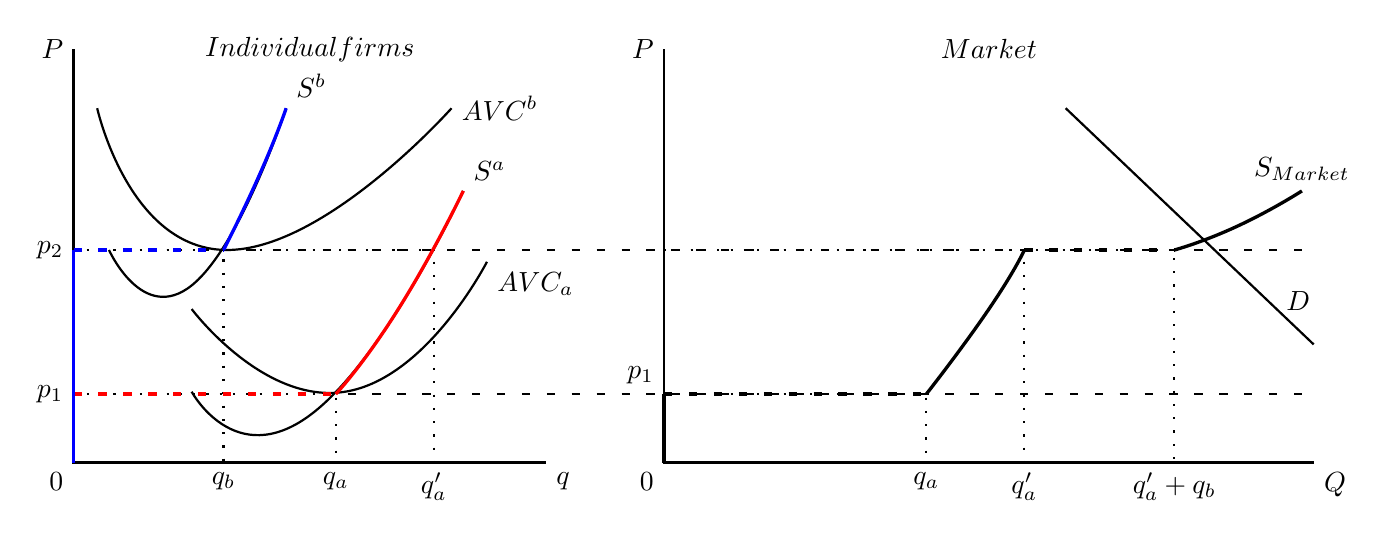
\begin{tikzpicture}[thick,font=\sffamily,scale=1.5]
	%axis and labels----------------------------
	 \draw (0,3.5) node[left]{$P$} -- (0,0) node[below left] {$0$} -- (4,0) node[below right]{$q$};
	   \draw (5,3.5) node[left]{$P$} -- (5,0) node[below left] {$0$} -- (10.5,0) node[below right]{$Q$};
	   \node[] at (2,3.5) {$Individual firms$}; %Firm label  
	   \node[] at (7.75,3.5) {$Market$}; %Market label  
	%Firm--------------------------------------
		%graphs	
		\draw[] plot [smooth, tension=1] coordinates {(1,1.3) (2.3,0.6) (3.5,1.7)}; %AVCa
		\draw[] plot [smooth, tension=1] coordinates {(1,0.6) (2,0.4) (3.3,2.3)}; %MCa
		\draw[] plot [smooth, tension=1] coordinates {(0.2,3) (1.3,1.8) (3.2,3)}; %AVCb
		\draw[] plot [smooth, tension=1] coordinates {(0.3,1.8) (1,1.5) (1.8,3)}; %MCb
		
		%dotted lines
		\draw[loosely dotted] (0,0.58) node[left]{$p_{1}$} -| node[pos=0.25,below=3mm] {} (2.22,0) node[below]{$q_{a}$}; %Dotted lines a1
		\draw[loosely dotted] (0,1.8) node[left]{} -| node[pos=0.25,below=3mm] {} (3.05,0) node[below]{$q^{\prime}_{a}$}; %Dotted lines a2
		\draw[loosely dashed] (0,0.58) -- (10.5,0.58); %p line
		\draw[loosely dotted] (0,1.8) node[left]{$p_{2}$} -| node[pos=0.25,below=3mm] {} (1.27,0) node[below]{$q_{b}$}; %Dotted lines b
		\draw[loosely dashed] (0,1.8) -- (10.5,1.8); %p line
		
		%Firm a supply curve	
		\draw[very thick, red] (0,0) -- (0,0.58); %part 1
		\draw[very thick, red, loosely dashed] (0,0.58)--(2.22, 0.58); %part 2
		\draw[very thick, red] plot [smooth, tension=1] coordinates{(2.22, 0.58) (2.75,1.3) (3.3,2.3)}; %part 3
		
		%Firm b supply curve	
		\draw[very thick, blue] (0,0) -- (0,1.8); %part 1
		\draw[very thick, blue, loosely dashed] (0,1.8)--(1.27, 1.8); %part 2
		\draw[very thick, blue] plot [smooth, tension=1] coordinates{(1.27,1.8) (1.58, 2.45) (1.8,3)}; %part 3
	
		%labels
		\node[above right] at (3.3,2.3) {$S^{a}$}; %firm supply label 
		\node[above right] at (1.8,3) {$S^{b}$}; %firm b supply label 
		\node[below right] at (3.5,1.7) {$AVC_{a}$}; %AVC a label
		\node[right] at (3.2,3) {$AVC^{b}$}; %AVC b label 
	
	%Market------------------------------------
		%Demand
		\draw[] (8.4,3) -- (10.5,1);
				
		%Market supply curve	
		\draw[very thick] (5,0) -- (5,0.58); %part 1
		\draw[very thick, loosely dashed] (5,0.58)--(7.22, 0.58); %part 2
		\draw[very thick] plot [smooth, tension=1] coordinates{(7.22, 0.58) (7.75,1.3) (8.05,1.8)}; %part 3
		\draw[very thick, loosely dashed] (8.05,1.8)--(9.32, 1.8); %part 4
		\draw[very thick] plot [smooth, tension=1] coordinates{(9.32, 1.8) (9.85,2) (10.4,2.3)}; %part 5
		
		%dotted lines
		\draw[loosely dotted] (5,0.58) node[above left]{$p_{1}$} -| node[pos=0.25,below=3mm] {} (7.22,0) node[below]{$q_{a}$}; %Dotted lines a
		\draw[loosely dotted] (5,1.8) node[left]{} -| node[pos=0.25,below=3mm] {} (8.05,0) node[below]{$q^{\prime}_{a}$}; %Dotted lines 2
		\draw[loosely dotted] (5,1.8) node[left]{} -| node[pos=0.25,below=3mm] {} (9.32,0) node[below]{$q^{\prime}_{a}+q_{b}$}; %Dotted lines 2
		
		%labels
		\node[above] at (10.4,2.3) {$S_{Market}$}; %Market supply label  
		\node[above right] at (10.18,1.2) {$D$}; %Demand supply label  
	
\end{tikzpicture}
\end{document}